%!TEX root = ../dissertation.tex

\chapter{Introduction}
\label{chapter:introduction}

Recently, the field of \gls{HRI} has been paying close attention to group interactions \cite{jung2017robots}. They refer to multi-party settings that extend dyads of one person and one robot, to cases where there are multiple people and/or multiple robots. The complexity of those settings lies on the non-linearity of the group processes, which is established on top of interdependent individual processes \cite{wildschut2007explanations}. The motivation behind this research topic arises from the natural and biological tendency that we, i.e. humans, have to live and organise ourselves in groups. It is reflected in the way our society is distributed and it also shapes our interactions with technology in general. Consequently, as robotic systems become part of our lives in various domains or environments, e.g. domestic \cite{christensen2003intelligent}, industrial \cite{guiochet2017safety}, public spaces \cite{jensen2005robots,kanda2009affective}, education \cite{belpaeme2018social}, health \cite{breazeal2011social}, they are naturally expected to engage in group settings or even integrate teams along with humans.



\begin{figure}[ht]
    \centering
    \begin{subfigure}[b]{0.3\textwidth}
        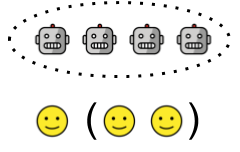
\includegraphics[width=\textwidth]{images/introduction/groups-robots.png}
        \caption{Groups of robots}
        \label{fig:groups-robots}
    \end{subfigure}
    \begin{subfigure}[b]{0.3\textwidth}
        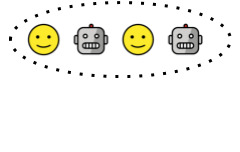
\includegraphics[width=\textwidth]{images/introduction/mixed-groups.png}
        \caption{Human-robot mixed groups}
        \label{fig:mixed-groups}
    \end{subfigure}
    \begin{subfigure}[b]{0.3\textwidth}
        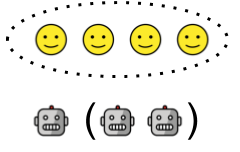
\includegraphics[width=\textwidth]{images/introduction/groups-humans.png}
        \caption{Robots near groups of humans}
        \label{fig:groups-humans}
    \end{subfigure}
    \caption{Structures of human-robot group interactions}
    \label{fig:group-interactions}
\end{figure}

\textcolor{blue}{Studying group interactions between humans and robots opens a wide range of challenges according to the nature and structure of those groups. We identified three distinct configurations of groups, see Figure~\ref{fig:group-interactions}, that lead to different types of interactions with robots. In Figure~\ref{fig:groups-robots}, \textit{groups of robots} represent the scenarios in which robots are expected to perform a task together around humans. The challenges in those situations may include exploring coordinated behaviour \cite{admoni2013dancing} or understanding how humans perceive robots in groups \cite{fraune2014negative}. In Figure~\ref{fig:mixed-groups}, \textit{human-robot mixed groups} depict scenarios in which robots act collaboratively alongside humans with similar goals. The challenges in those situations are usually focused on enhancing the collaboration and may range from signaling behaviour \cite{jung2013engaging} to support telepresence \cite{stoll2018wait}. Finally, in Figure~\ref{fig:groups-humans}, \textit{robots near groups of humans} illustrate scenarios in which the robot is required to act near a group of humans without being part of that group. The challenges may overlap with the mixed-groups, especially if the role of the robot is to provide assistance or facilitate the interaction. In those cases, the robot can also have a strong impact on the interaction among humans \cite{jung2018robot}. Examples of other challenges may include, for instance, the detection of group patterns \cite{leite2015comparing}.}



\textcolor{blue}{Overall, these research challenges contribute to successfully integrate robots in a society that is organised in groups. Robots will, therefore, be required to act in groups, to be part of groups alongside humans, or to be close to groups of humans. Jung and collaborators have proposed three broad research avenues to advance the study of group interaction in \gls{HRI} \cite{jung2017robots}. Firstly, understanding how the dynamics of existing group settings is shaped by a robot. In other words, analysing the impact robots have on the group processes, e.g. conflict or power. Secondly, understanding how the actual human-human interaction is influenced by robots. Finally, the last research avenue matches exactly the focus of this dissertation, which is how can robots mediate or enhance the performance of work groups or teams.}


\section{Group Dynamics}
As research on group interaction between humans and robots is still in its infancy, insights from other behavioural fields must be considered. In particular, the scientific study of all the processes that occur within and between interpersonal groups is called \textit{group dynamics}, which is being explored for the past century by several disciplines within the social sciences, e.g. organisational behaviour, social psychology, or management.

The social psychologist Forsyth defined a group as \textit{``two or more individuals who are connected by and within social relationships''} \cite{forsyth1990group}. He also pointed out the five main qualities of groups ---interaction, goals, interdependence, structure and cohesion--- and the fact that each one of them provides complex and fascinating phenomena when analysed more closely. According to these key qualities, a group interacts or sustains a relationship in order to achieve a certain purpose or outcome. It is usually structured in a way that its members have interdependent roles or relations that remain together due to a cohesive alliance. There is, however, a particular type of groups that intensifies these five qualities to an extreme level ---teams. Members of a team are usually committed to a common goal in which the individual success is only a consequence of the collective success. There is a strong interdependence of their efforts that requires a coordinated interaction. In terms of structure, teams usually present highly adaptive skills that allow a revision of their norms and procedures in order to improve their functioning. Finally, the cohesive alliance of a team is also a salient characteristic, as Forsyth defines teams as \textit{``unified, cohesive groups''}.



\section{Research Problem}
As previously mentioned, teams are a particularly strong type of groups, in the sense that members of a team experience intense relations towards their shared goal. Nevertheless, as teamwork and collaboration do only require a team to have at least two entities, most \gls{HRI} literature in this topic is focused on dyadic collaborations \cite{hoffman2007effects,dragan2015effects,huang2016anticipatory,chang2018effects,shayganfar2019appraisal,hoffman2019evaluating}. The exploration of teamwork and collaboration within small groups of humans and robots (i.e. groups with more than one person and/or more than one robot) is still scarce \cite{fraune2017teammates}.

Although robots can easily outperform humans when individually executing specific tasks, e.g. \cite{butner2003transforming} or \cite{cicconet2012visual}, achieving satisfactory and effective collaborations might not be straightforward \cite{bauer2008human}. As soon as robots start working close to humans or are required to collaborate with them, their social capabilities become not only useful but also necessary. Dautenhahn et al. extensively revisited the definition of socially embedded agents which are tightly coupled to the social environment \cite{dautenhahn2002embodied}. The authors further proposed these agents can ``benefit from possessing some degree of awareness of the social system, i.e. a means of perceiving and sensing structures within the social world, and means of acting within it''. This thesis aims at contributing to this notion of socially embeddedness, specifically in relation to the group dynamics of an environment where the robot is required to be a team member.



%argument why now measuring performance
An immediate question that might occur is: what exactly is \textit{the effectiveness} of a mixed human-robot team? An intelligible answer can be that it is highly dependent on task itself, the purpose or the goals of the team. Therefore, we acknowledge that there might be several different ways of assessing effectiveness. One possibility is maximising the performance achieved by the team, which is mostly the main motivation for developing robotic teammates. There are, however, other possibilities such as examining other aspects or factors that sustain the quality of the team and may, in turn, mediate performance. One of those factors is certainly cohesion, pointed by many authors as the most important aspect of groups and, consequently, of teams. It is considered the integrity, solidarity and unity that maintains a group together or, in other words, the ``groupiness of a group''. Cohesion is associated with satisfaction, performance, and productivity. For instance, Mullen and Cooper found an interesting bidirectional relationship between cohesion and performance, which suggests that not only cohesive teams tend to perform better, but also the success of the team leads to increased cohesion \cite{mullen1994relation}.


Additionally, there are many complex tasks in which the performance or the outcome achieved by the team is affected, or even damaged, by external factors. And yet, the integrity of a team may be strong enough to sustain satisfaction and the \textit{esprit de corps} in those situations. As a result, we are interested in this particular type of cohesive alliance in mixed teams of humans and robots and we have formulated our research problem as follows.

\begin{indented}
%In a mixed human-robot team setting, how can a social robot establish and improve a cohesive alliance with the other team members?%How can we create an effective robotic teammate? In particular, how are cohesive alliances established with robotic teammates and
How can we endow a social robot with the ability to improve the cohesive alliance in a team setting with humans?
\end{indented}

An initial consideration to undertake this research problem is the understanding of how humans establish cohesive alliances in their interpersonal groups or teams. The multi-dimensionality of the \textit{cohesion} construct suggests that there are five possible courses that lead to cohesiveness: the task, the social bonds, the collective entity, the structure and emotions. \textit{Task cohesion} emerges from the shared commitment towards a common goal, while \textit{social cohesion} develops from the attractions among the members. The identification of the members with the group and the degree of belonging constitutes the \textit{collective cohesion}. The \textit{structural cohesion} derives from the norms, roles and relationships that link the members of the group. Finally, \textit{emotional cohesion} is the intensity of the members to express group feelings. In this thesis, we will explore the first four types or dimensions of cohesion.

Overall, this research problem can be tackled in many different ways, especially considering the multi-dimensionality of the cohesion construct. Therefore, it is important to clarify what are the research directions that this dissertation will undertake. The challenges or goals that we address are twofold. On the one hand, (a) \textit{to evaluate the impact of the robot's social behaviours on the cohesion of the team}. This first research goal aims at understanding the evolution and development of teams with humans and robots. It includes the analysis of how do people perceive the robotic teammate, how does the behaviour of the robot influence the team, or even how do external factors affect those perceptions. On the other hand, (b) \textit{to develop computational mechanisms to autonomously increase the cohesive alliance of a mixed team of humans and robots}. This second research goal is focused on the computational aspects that facilitate the robotic agent to autonomously improve the cohesion of its team. These mechanisms may affect both its decision-making and its perceptive skills to analyse and model the group.



\section{Contributions}
This dissertation holds four major contributions that address the two aforementioned goals:

\begin{itemize}
    \item[1.] \textbf{Evaluate the impact of the robot's social behaviours on the social cohesion of the team} - Social cohesion develops from the attractions of group members both at individual- and group-level. Those attractions can flourish when team members have particular traits, for instance. However, what exactly are the traits that we seek in robotic teammates? Based on the learning-goal theory, we created two distinct characters for social robots to either express a performance goal or a learning goal, which translate into more competitive or more relationship-driven behaviours. We conducted a user study using a card-game where human players could form a team with each robotic character. By exploring different team formations, we contribute to the understanding of membership preferences towards robotic teammates, which is detailed in Chapter~\ref{chapter:membership-formation}.
    
    
    \item[2.] \textbf{Evaluate the impact of the team's outcome on the collective cohesion} - Collective cohesion reflects the degree of identification with the group. It is usually mentioned as the replacement of the ``I'' by the ``we'' and, when this feeling becomes stronger, it may even affect one's actions with the collective goals taking priority over the individual ones. We aim at exploring how people perceive different levels of collective cohesion on robotic teammates and how those are influenced by the achieved outcome being positive or negative. Chapter~\ref{chapter:pro-sociality} presents a user study that explores this research question in a Public Goods Game between a mixed team of one human and two robots. The results contribute with important considerations to the understanding of collective cohesion in teams of humans and robots.
    
    \item[3.] \textbf{Develop computational mechanisms for the robotic teammate to improve collective cohesion} - According to the group identity theory, there is a group of emotions that reflects a high level of identification with the group, which are called the \textit{group-based emotions}. Chapter~\ref{chapter:group-based-emotions} describes a computational approach to implement the group identity theory on an emotional agent in order to express this type of emotions. It also contributes with a user study that evaluates the proposed model on a robotic teammate and its impact on the collective cohesion of the team.
    
    \item[4.] \textbf{Develop computational mechanisms for the robotic teammate to autonomously perceive the structural cohesion of the team} - The structure of a team can be represented in a graph where nodes correspond to the team members and the links may identify different types of relations, such as roles, norms, or interactions. Usually, the density and topology of those structures is associated with the degree of cohesion of a team. We plan to extend the perceptive skills of a social robot to detect the communication network of the team members. Such mechanism will allow the robotic teammate to autonomously perceive aspects of the group related with its structural cohesion. Chapter~\ref{chapter:future-work} proposes an approach to address this last contribution of this dissertation.
\end{itemize}



\section{Roadmap}
The current document contains 7 chapters and is organised as follows. %\textbf{Chapter~\ref{chapter:background}} provides relevant and central notions on interpersonal cohesion, which will support the further reading of the current document. 
In \textbf{Chapter~\ref{chapter:related-work}}, we present the state-of-the-art on group interactions between humans and robots. The following three chapters, \textbf{Chapter~\ref{chapter:membership-formation}}, \textbf{Chapter~\ref{chapter:pro-sociality}}, and \textbf{Chapter~\ref{chapter:group-based-emotions}}, detail our previous work, corresponding to contributions 1, 2 and 3, respectively. The fourth and last contribution corresponds to the future work of this ongoing dissertation and the proposed approach to address it is presented in \textbf{Chapter~\ref{chapter:future-work}}.

Finally, the document ends in \textbf{Chapter~\ref{chapter:conclusion}} with a discussion and concluding remarks on the current contributions of this thesis and a proposal to address our last research goal 2.2, that constitutes our on-going work.
